\let\negmedspace\undefined
\let\negthickspace\undefined
\documentclass[journal]{IEEEtran}
\usepackage[a5paper, margin=10mm, onecolumn]{geometry}
%\usepackage{lmodern} % Ensure lmodern is loaded for pdflatex
\usepackage{tfrupee} % Include tfrupee package

\setlength{\headheight}{1cm} % Set the height of the header box
\setlength{\headsep}{0mm}     % Set the distance between the header box and the top of the text

\usepackage{gvv-book}
\usepackage{gvv}
\usepackage{cite}
\usepackage{amsmath,amssymb,amsfonts,amsthm}
\usepackage{algorithmic}
\usepackage{graphicx}
\usepackage{textcomp}
\usepackage{xcolor}
\usepackage{txfonts}
\usepackage{listings}
\usepackage{multicol}
\usepackage{enumitem}
\usepackage{mathtools}
\usepackage{gensymb}
\usepackage{comment}
\usepackage[breaklinks=true]{hyperref}
\usepackage{tkz-euclide} 
\usepackage{listings}
% \usepackage{gvv}                                        
\def\inputGnumericTable{}                                 
\usepackage[latin1]{inputenc}                                
\usepackage{color}                                            
\usepackage{array}                                            
\usepackage{longtable}                                       
\usepackage{calc}                                             
\usepackage{multirow}                                         
\usepackage{hhline}                                           
\usepackage{ifthen}                                           
\usepackage{lscape}
\usepackage{tikz}
\usetikzlibrary{patterns}

    
\begin{document}

\bibliographystyle{IEEEtran}
\vspace{3cm}


\title{2011-ME-'1-13'}
\author{EE24BTECH11023}
%\maketitle
%\newpage
%\bigskip

{\let\newpage\relax\maketitle}

\renewcommand{\thefigure}{\theenumi}
\renewcommand{\thetable}{\theenumi}
\setlength{\intextsep}{10pt} % Space between text and floats


\numberwithin{equation}{enumi}
\numberwithin{figure}{enumi}
\renewcommand{\thetable}{\theenumi}
\begin{large}

\text{Q.1-Q.25 Carry one mark each}
\end{large}
    \begin{enumerate}
        \item A streamline and an equipotential line in a flow field
    
    \begin{multicols}{2}
    
    
    \begin{enumerate}
    
        \item are parallel to each other
        \item are perpendicular to each other
        \item intersect at an angle
        \item are identical
    \end{enumerate}
    \end{multicols}
     \item If a mass of moist air in an airtight vessel is heated to a higher temperature,then
         \begin{multicols}{2}

    \begin{enumerate}
        \item specific humidity of the air increases
        \item specific humidity of the air decreases
        \item relative humidity of the air increases
        \item relative humidity of the air decreases

    \end{enumerate}
        \end{multicols}

    \item In a condenser of a power plant,the steam condenses at a temperature $60^{\circ}$C.The cooling water enters at $30^{\circ}$C and leaves at $45^{\circ}$C.The logarithmic mean temperature difference (LMTD) of the condenser is
        \begin{multicols}{2}

    \begin{enumerate}
        \item $16.2^{\circ}$C
        \item $21.6^{\circ}$C
        \item $30^{\circ}$C
        \item $37.5^{\circ}$C

        
        \end{enumerate}
            \end{multicols}

        \item A simply supported beam PQ is loaded by a moment of 1 kN-m at the mid-span of the beam as shown in the figure.The reaction forces $R_{P}$ and $R_{Q}$ at the supports P and Q respectively are

      \begin{figure}[H]
        \centering
        

    \begin{tikzpicture}
        \begin{axis}[
            axis lines = middle,
            xlabel = $I_f$,
            ylabel = $V_{oc}$,
            xmin = 0, xmax = 5,
            ymin = 0, ymax = 450,
            xtick = {0,1,2,3,4},
            ytick = {0,100,200,300,400},
            x label style={at={(axis description cs:1,0)},anchor=west},
            y label style={at={(axis description cs:0,1)},anchor=south},
            extra x ticks={0},
            extra y ticks={0},
            extra tick style={grid=major},
            axis line style=thick,
            xlabel near ticks,
            ylabel near ticks,
            every axis plot/.append style={thick},
            legend pos = north west,
            width=10cm, height=8cm,
        ]

        % Plot for OCC curve
        \addplot[domain=1.09:4, samples=100, smooth] {100*(x-1.03)^(0.5)+250};

        % Plot for SCC curves
        \addplot[domain=0:2, samples=2] {25*x};
        \addplot[domain=0:1.12, samples=2] {250*x};

        % Points with labels
        \node at (axis cs:0,0) [below left] {\small $(0,0)$};
        \node at (axis cs:0,10) [left] {\small $(0,10)$};
        \node at (axis cs:1,110) [above left] {\small $(1,110)$};
        \node at (axis cs:2,210) [above left] {\small $(2,210)$};
        \node at (axis cs:4,20) [below right] {\small $(4,20)$};
        \node at (axis cs:4,400) [above] {\small $(8,400)$};

        % Additional labels for OCC and SCC curves
        \node at (axis cs:3.5,350) [above] {OCC};
        \node at (axis cs:1.2,30) [below right] {SCC};

        % Right-hand axis line and label
        \draw[->, thick] (axis cs:4.8,0) -- (axis cs:4.8,450) node [right] {$I_{sc}$};

        % Top axis label for V_oc
        \node[above] at (axis cs:0,450) {$V_{oc}$};

        \end{axis}
    \end{tikzpicture}
   
  % Use the correct path to your Q4.tex file
    \end{figure}
       




    \begin{multicols}{2}

        \begin{enumerate}
    \item 1 kN downward, 1 kN upward
    \item 0.5 kN upward, 0.5 kN downward
    \item 0.5 kN downward, 0.5 kN upward
    \item 1 kN upward, 1 kN upward

     \end{enumerate}
         \end{multicols}

     \item A double-parallelogram mechanism is shown in the figure.Note that PQ is a single link.the mobility of the mechanism is

      \begin{figure}[H]
        \centering
        
    \begin{tabular}{cc}
        \toprule
        \( f \) (MPa) & Number of specimens with \\
                      & compressive strength equal to \( f \) \\
        \midrule
        23   & 4 \\
        28   & 2 \\
        22.5 & 5 \\
        31   & 5 \\
        29   & 4 \\
        \bottomrule
    \end{tabular}
  % Use the correct path to your Q4.tex file
    \end{figure}
       



    \begin{multicols}{2}

         \begin{enumerate}
             \item $-1$
             \item $0$
             \item $1$
             \item $2$

\end{enumerate}
    \end{multicols}

     \item The maximum possible draft in cold rolling of sheet increases with the
         \begin{multicols}{2}

     \begin{enumerate}
         \item increase in coefficient of friction
         \item decrease in coefficient of friction
         \item decrease in roll radius
         \item increase in roll velocity
     \end{enumerate}
         \end{multicols}

     \item The operation in which oil is permeated into the pores of a powder metallurgy product is known as
         \begin{multicols}{2}

     \begin{enumerate}
         \item mixing
         \item sintering
         \item impregnation
         \item infiltration
     \end{enumerate}
         \end{multicols}

     \item A hole is of dimension  $\varnothing 9^{\genfrac{}{}{0pt}{}{+0.015}{+0}}$  mm.The corresponding shaft is of dimension $\varnothing 9^{\genfrac{}{}{0pt}{}{+0.010}{+001}}$ mm.The resulting assembly has
         \begin{multicols}{2}

     \begin{enumerate}
         \item loose running fit
         \item close running fit
         \item transition fit
         \item interference fit
         \end{enumerate}
             \end{multicols}

         \item Heat and work are
             \begin{multicols}{2}

         \begin{enumerate}
             \item intensive properties
             \item extensive properties
             \item point functions
             \item path functions
             \end{enumerate}
                 \end{multicols}

             \item A column has a rectangular cross-section of $10 mmx 20 mm$ and a length of 1 m.The slenderness ratio of the column is close to
                 \begin{multicols}{2}

             \begin{enumerate}
                 \item $200$
                 \item $346$
                 \item $477$
                 \item $1000$

             \end{enumerate}
                 \end{multicols}

             \item A series expansion for the function $\sin \theta$ is
                 \begin{multicols}{2}

             \begin{enumerate}
                 \item $ 1 - \frac{\theta^2}{2!} + \frac{\theta^4}{4!} - \cdots $
                 \item $ \theta - \frac{\theta^3}{3!} + \frac{\theta^5}{5!} - \cdots $
                 \item $ 1 + \theta + \frac{\theta^2}{2!} + \frac{\theta^3}{3!} + \cdots $
                 \item $ \theta + \frac{\theta^3}{3!} + \frac{\theta^5}{5!} + \cdots $

                 
             \end{enumerate}
                 \end{multicols}


\item Green sand mould indicates that         
\begin{multicols}{2}

             \begin{enumerate}
                 \item polymeric mould has been cured
                 \item mould has been totally dried
                 \item mould is green in colour
                 \item mould contains moisture

             \end{enumerate}
                 \end{multicols}

             
\item What is $\lim_{\theta \to 0} \frac{\sin \theta}{\theta}$ equal to?
    \begin{multicols}{2}

\begin{enumerate}
    \item $\theta$
    \item $\sin \theta$
    \item $0$
    \item $1$

    
\end{enumerate}
    \end{multicols}



\end{enumerate}

        
     
\end{document}